\documentclass[12pt]{article}
\usepackage[pdfborder={0 0 0.5 [3 2]}]{hyperref}%
\usepackage[left=1in,right=1in,top=1in,bottom=1in]{geometry}%
\usepackage[shortalphabetic]{amsrefs}%
\usepackage{amsmath}
\usepackage{enumerate}
\usepackage{enumitem}
\usepackage{amssymb}                
\usepackage{amsmath}                
\usepackage{amsfonts}
\usepackage{amsthm}
\usepackage{bbm}
\usepackage[table,xcdraw]{xcolor}
\usepackage{tikz}
\usepackage{float}
\usepackage{booktabs}
\usepackage{svg}
\usepackage{mathtools}
\usepackage{cool}
\usepackage{url}
\usepackage{graphicx,epsfig}
\usepackage{framed}
\usepackage{hyperref}  

\usetikzlibrary{automata,arrows,positioning,calc}
\DeclarePairedDelimiter\abs{\lvert}{\rvert}%
\DeclarePairedDelimiter\norm{\lVert}{\rVert}%
\DeclarePairedDelimiter\ceil{\lceil}{\rceil}
\DeclarePairedDelimiter\floor{\lfloor}{\rfloor}

\makeatletter
\renewcommand*\env@matrix[1][*\c@MaxMatrixCols c]{%
  \hskip -\arraycolsep
  \let\@ifnextchar\new@ifnextchar
  \array{#1}}
\makeatother

\newtheorem{theorem}{Theorem}[section]
\newtheorem{corollary}{Corollary}[theorem]
\newtheorem{proposition}[theorem]{Proposition}
\newtheorem{lemma}[theorem]{Lemma}

\theoremstyle{definition}
\newtheorem{definition}[theorem]{Definition}
\newtheorem{exercise}{Exercise}%
\newtheorem{problem}[exercise]{Problem}%
\newtheorem*{example}{Example}

\theoremstyle{remark}
\newtheorem*{question}{Question}
\newtheorem*{observation}{Observation}
\newtheorem*{remark}{Remark}

\graphicspath{ {images/} }

\setlength{\parindent}{0cm}
\renewcommand{\vec}[1]{\ensuremath{\mathbf{#1}}}

\def\noi{\noindent}
\def\T{{\mathbb T}}
\def\R{{\mathbb R}}
\def\N{{\mathbb N}}
\def\C{{\mathbb C}}
\def\Z{{\mathbb Z}}
\def\P{{\mathbb P}}
\def\E{{\mathbb E}}
\def\Q{\mathbb{Q}}
\def\ind{{\mathbb I}}

\def\cale{{\mathcal E}}
\def\cals{{\mathcal S}}
\def\calc{{\mathcal C}}
\def\caln{{\mathcal N}}
\def\calb{{\mathcal B}}
\def\calg{{\cal G}}

\def\ds{\displaystyle}
\def\ra{\rightarrow}
\newcommand{\conv}{\mbox{\rm conv}}
\newcommand{\spaan}{\mbox{\rm span}}
\newcommand{\deet}{\mbox{\rm det}}
\newcommand{\aff}{\mbox{\rm aff}}
\newcommand{\cl}{\mbox{\rm cl}}
\newcommand{\dimm}{\mbox{\rm dim}}
\newcommand{\sm}{\setminus}
\def\ci{\perp\!\!\!\perp}

\newcommand{\ink}{\rule{.5\baselineskip}{.55\baselineskip}}

\begin{document}

\setcounter{section}{1}
\section{Discrete Random Variables}

\subsection{Random Variables}
A \emph{random variable} is a real-valued function on a sample space\footnote{It's not really a variable at all, but we are stuck with the terminology.}. A random variable generally is a quantity we wish to measure; the output of the random variable depends on which element of the sample space is chosen. In this section, we will look at discrete random variables.

\begin{framed}
A \emph{discrete} random variable $Y$ is a random variable which can only take on a finite or countable set of distinct values.
\end{framed}

Here are some examples of discrete random variables:
\begin{enumerate}
\item The number of voters in Rhode Island who prefer Hillary Clinton.
\item The number of defective lightbulbs out of a shipment of 1000 lightbulbs.
\item The number of times I play a slot machine in Las Vegas until I win.
\end{enumerate}

We will use the following simple example to illustrate features of discrete random variables.

\begin{example}Let $\cals$ be the sample space representing the flip of two fair coins. Let $Y$ be the number of heads flipped. Then $Y$ is a discrete random variable, since it can only have the values 0, 1, or 2. We can illustrate it graphically below.
\begin{figure}[H]
\centering
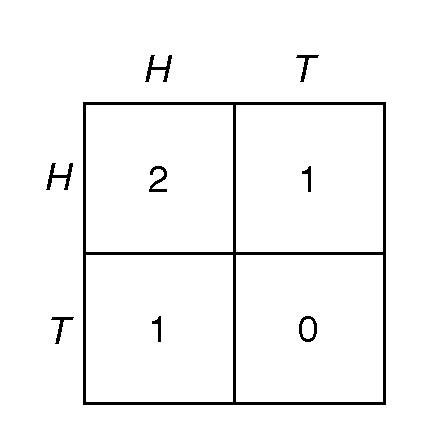
\includegraphics[width=3cm]{numberofheads.eps}
\end{figure}
\end{example}

Uppercase letters, such as $Y$, are used to designate random variables. We use lowercase letters, such as $y$, to designate a value that a random variable can take. The expression $(Y = y)$ is shorthand for the set of all points in our sample space $\cals$ for which the random variable $Y$ outputs the value $y$. Since $(Y = y)$ is a subset of $\cals$, it is an event in our sample space. In the two-coin-toss problem, for example, the possible values of $Y$ are 0, 1, and 2, so we have:
\begin{itemize}[noitemsep]
\item $(Y = 0) = \{ (T, T) \}$
\item $(Y = 1) = \{ (H, T), (T, H) \}$
\item $(Y = 2) = \{ (H, H) \}$
\end{itemize}

Since $(Y = y)$ is an event in our sample space, we can talk about its probabiltiy, i.e. $\P(Y = y)$. In fact, the point of random variables is to do just this! 

\begin{framed}
  \emph{Probability of a discrete random variable }\\
  \rule{\dimexpr\linewidth-2\fboxsep-2\fboxrule}{.1pt} \\
  The probability that a discrete random variable $Y$ takes the value $y$, denoted $\P(Y = y)$, or $p(y)$ for short, is the probability of the event $(Y = y)$, the set of all points in the sample space $\cals$ which output the value $y$. \\

  $\P(Y = y)$ is the sum of the probabilities of all the simple events in $\cals$ which are assigned the value $y$ by the random variable $Y$.
\end{framed}

Back to our two-coin-toss problem, let's look at the probabilties of the random variable $Y$. For convenience, here is a picture of the sample space probabilities next to a graphical representation of $Y$. Since we are using the discrete uniform distribution for coin tosses, each simple event in our sample space has probability 1/2.
\begin{figure}[H]
\centering
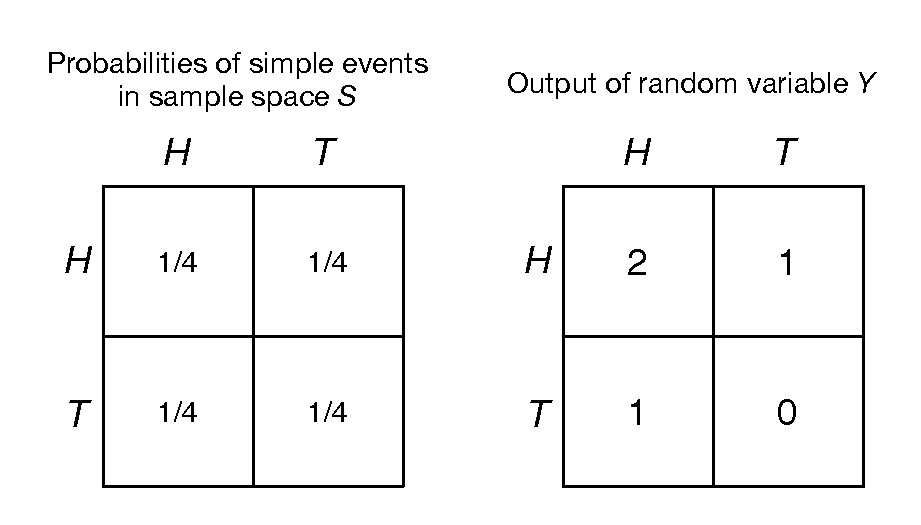
\includegraphics[width=8cm]{numberofheads2.eps}
\end{figure}

Using the rule above, we can compute the following probabilties for $Y$ by adding up the probabilities of the underlying simple events. In this case, since we are using the discrete uniform distribution, we could also just count the number of simple events which lead to each output of $Y$ and divide by 4, the size of the sample space.
\begin{itemize}[noitemsep]
\item $\P(Y = 0) = 1/4$
\item $\P(Y = 1) = 1/4 + 1/4 = 1/2$
\item $\P(Y = 2) = 1/4$
\end{itemize}

\begin{framed}
  \emph{Probability mass function }\\
  \rule{\dimexpr\linewidth-2\fboxsep-2\fboxrule}{.1pt} \\
  The \emph{probablity mass function (pmf)} is a function which gives the probabiltiy that a discrete random variable $Y$ is exactly equal to a value $y$. The pmf can be represented as a function, table, or graph which gives the values $p(y) = \P(Y = y)$ for all possible values $y$ which $Y$ can take.
\end{framed}

In the two-coin-flip example, we can represent the pmf of $Y$ in a table:
\begin{figure}[H]
\centering
\begin{tabular}{l@{\hskip 2cm}l}
\toprule
$y$ & $p(y)$\\
\midrule
0 & 1/4\\
1 & 1/2\\
2 & 1/4\\
\bottomrule
\end{tabular}
\end{figure}

We can also represent the pmf graphically as a histogram\footnote{I will undoubtedly lose some of my math street cred if I admit to using Microsoft Excel for these histograms, but in some cases it really is the easiest tool to use.}.
\begin{figure}[H]
\centering
\includegraphics[width=5cm]{2coinshisto}
\end{figure}


A discrete random variable induces a probability distribution on the sample space of all possible values the random variable can take. This is a different sample space from the original sample space. Back to our two-coin-flip example, the random variable $Y$ induces a probability distribution on a new sample space $\mathcal{T} = \{0, 1, 2\}$. The probabilities of the sample points in $\mathcal{T}$ are the probabilties $p(y)$ for $y = 0, 1, 2$. We can illustrate this new sample space in a picture.

\begin{figure}[H]
\centering
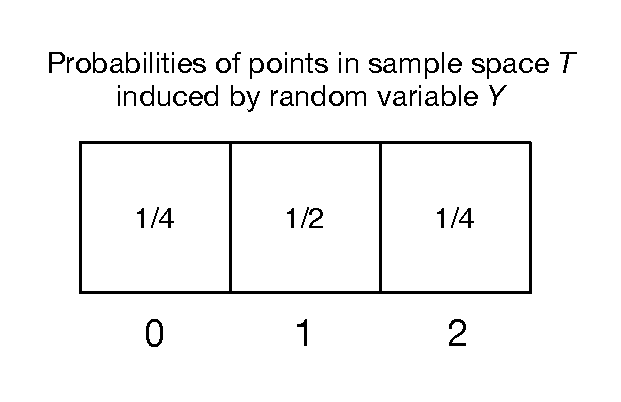
\includegraphics[width=5cm]{induced1.eps}
\end{figure}

Often (as we shall see), we care much more about the sample space induced by a random variable than the underlying sample space. Since a discrete random variable induces a probability distribution, the following must be true.

\begin{framed}
For any discrete random variable $Y$:
\begin{align*}
0 \leq p(y) &\leq 1 \:\text{ for all }y \\
\sum_{\text{all } y} p(y) &= 1
\end{align*}
where $p(y) = \P(Y = y)$. Since we have a discrete sample space, the sum is finite or countable.
\end{framed}

Let's look at two more examples, this time involving the rolls of two six-sided dice.

\begin{example}Let $\cals$ be the sample space representing the rolls of two six-sided dice. Consider the following two random variables:
\begin{enumerate}
\item $X$ = the sum of the two dice
\item $Y$ = the larger of the two die rolls (if they are the same, then it's just equal to both die rolls)
\end{enumerate} 
Let's look at these random variables graphically.
\begin{figure}[H]
\centering
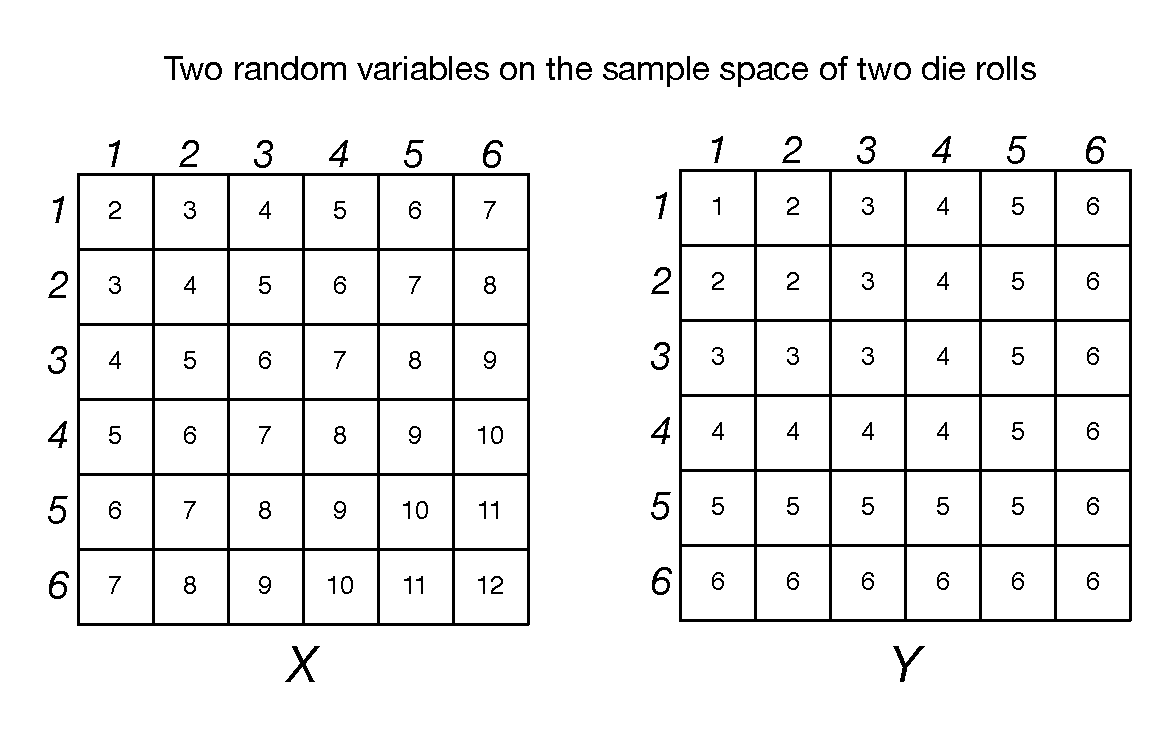
\includegraphics[width=10cm]{2dicervs.eps}
\end{figure}

The random variable $X$ induces a probability distribution on the set of integers $\{2, 3, 4, \dots, 12\}$, and the random variable $Y$ induces a probability distribution on the set of integers $\{1, 2, 3, 4, 5, 6\}$. Let's look at the pmfs of both random variables using histograms.

\begin{figure}[H]
\centering
\includegraphics[width=7cm]{sumoftwodice.pdf}
\includegraphics[width=7cm]{maxoftwodice.pdf}
\end{figure}
Both of these distributions are nonuniform, even though the underlying distribution of the two dice is uniform. The first distribution, that of the random variable $X$, is a familiar one to afficionados of board games such at Settlers of Catan and Monopoly. We can also write the pmfs in table form. For the random variable $Y$, we have:
\begin{figure}[H]
\centering
\begin{tabular}{l@{\hskip 2cm}l}
\toprule
$y$ & $p(y)$\\
\midrule
1 & 1/36\\
2 & 3/36\\
3 & 5/36\\
4 & 7/36\\
5 & 9/36\\
6 & 11/36\\
\bottomrule
\end{tabular}
\end{figure}
The pmf for $X$ can be expressed similarly.
\end{example}

\subsection{Expected Value}
Given a discrete random variable, we can definite it's mean, or expected value. 

\begin{framed}
  \emph{Expected value of a random variable}\\
  \rule{\dimexpr\linewidth-2\fboxsep-2\fboxrule}{.1pt} \\
For a discrete random variable $Y$ with probability function $p(y)$, the \emph{expected value} or \emph{mean} is defined to be
\[
\E(Y) = \sum_{\text{all }y}y\:p(y)
\]
where the sum is taken over all possible values $y$ can take. We can think of the expected value as a weighted average of the values of $Y$ with each possible output $y$ weighted by its probability $p(y)$. The expected value is sometimes written as $\mu$ (for mean)
\end{framed}

Here is one interpretation of the expected value of a random variable. Think of a random variable $Y$ as an observation from an experiment. Suppose we perform the experiment $n$ times, and observe $n$ values of $Y$, which we shall designate $y_1, y_2, \dots, y_n$. Then for large $n$,
\[
\frac{y_1 + y_2 + \cdots + y_n}{n} \approx \E(Y)
\]
where the approximation ``gets better'' as $n$ gets larger, i.e. as we perform more experiments. The quantity on the left hand side is known as the \emph{empirical mean} or \emph{sample mean} and looks like what we likely learned in high school (add a bunch of stuff up and divide by the number of things). The expected value is, in a sense, the limit of the empirical mean as the sample size approaches infinity. We will make this more precise later in the course, but this is a good concept to keep in mind.

\begin{example}Let $X$ represent the roll of a standard, fair six-sided die. (In this case, the underlying sample space is $\cals = \{1, 2, 3, 4, 5, 6\}$ with the discrete uniform distribution, and the random variable $X$ is the same as the sample space element selected.) Then the expected value of $X$ is:
\begin{align*}
\E(X) &= \sum_{x = 1}^6 x \P(X = x) \\
&= \sum_{x = 1}^6 x \frac{1}{6} \\
&= \frac{1}{6 } \sum_{x = 1}^6 x \\
&= \frac{21}{6} \\
&= 3.5
\end{align*}
where used the fact from the discrete uniform distribution that $\P(X = x)$ = 1/6 for all $x$. Note that the expected value of 3.5 is not a possible value of $X$, i.e. we cannot roll a 3.5 on a single die. Given our ``long term average'' interpretation, this is saying that we expect the empirical average to approach 3.5 as the number of rolls increases, not that a 3.5 is the most likely die roll.
\end{example}

\begin{example}Let $Y$ be the random variable above representing the maximum of two dice. What is the expected value of $Y$.\\

To find the expected value, we do a weighted average using the probabities in the table above.
\begin{align*}
\E(Y) &= \sum_{y = 1}^6 y \P(Y = y) \\
&= 1 \cdot \frac{1}{36} + 2 \cdot \frac{3}{36} + 3 \cdot \frac{5}{36} + 4 \cdot \frac{7}{36} + 5 \cdot \frac{9}{36} + 6 \cdot \frac{11}{36} \\
&= \frac{1 + 6 + 15 + 28 + 45 + 66}{36} \\
&= \frac{161}{36} \approx 4.47
\end{align*}
\end{example}

\subsection{Properties of Expectation}
We will discuss several properties of the expected value. The first and and one of the most important is the \emph{linearity of expectation}.

\begin{framed}
  \emph{Linearity of expectation}\\
  \rule{\dimexpr\linewidth-2\fboxsep-2\fboxrule}{.1pt} \\
Let $X$ and $Y$ be two random variables\footnote{So far we have only discussed what an expected value is in terms of discrete random variables, but this is true for all random variable.}, and let $a$ and $b$ be constants. Then
\[
\E(aX + bY) = a\E(X) + b\E(Y)
\]
This is called \emph{linearity} in reference to linear algebra, i.e. we can separate addition and pull out constants. This holds whether or not $X$ and $Y$ are independent. \\

As a corollary of this, if we have random variables $X_1, X_2, \dots, X_n$, then
\[
\E(X_1 + X_2 + \cdots + X_n) = \E(X_1) + \E(X_2) + \cdots + \E(X_n)
\]
\end{framed}

Linearity of expectation is a really nice property since it does not require the random variables to be independent. Let's do a problem to illustrate the usefulness of linearity of expectation.

\begin{example}
One evening, $n$ customers dine at a restaurant. Each gives their hat to a hat-check person at a restaurant. (These are fashionable diners!) After dinner, the hat-check person gives the hats back to the customers in a random order, i.e. each customer receives one of the hats uniformly at random. What is the expected number of customers that get their own hat back?\\

Let $X$ be the number of customers who get their own hat back. Then $X$ is a discrete random variable taking values $0, 1, \dots, n$. By the definition of expected value:
\[
\E(X) = \sum_{i = 1}^n i \:\P(X = i)
\]
At this point, we have a mess! We have to compute $\P(X = i)$ for all $i$, which would involve a sophisticated combinatorial argument, as well as considerable time and mental energy. Luckily for us, there is another way.\\

We will use the method of indicator random variables, together with linearity of expectation, to solve this problem. An \emph{indicator random variable} is a random variable $I$ which only takes the values 0 and 1. It is used to indicate whether (or not) an event takes place: $I = 1$ if the event happens, and $I = 0$ if the event does not happen.\\

We will define some indicator random variables for this problem. First, let's number the customers $1, 2, \dots, n$.
For $i = 1, \dots, n$, let $X_i$ be the indicator random variable for the event that customer $i$ gets their own hat back. In other words,
\[
X_i = \begin{cases}1 & \text{customer $i$ gets their own hat back}\\
0 & \text{otherwise}\end{cases}
\]

From the way we have constructed these indicator random variables, we see that
\[
X = X_1 + X_2 + \cdots + X_n
\]
Does this make sense? If we add up the indicator random variables, we are adding a 1 whenever a customer gets their own hat back, which gives us the total number of customers who get their hat back. Now we use linearity of expectation. The indicator variables $X_i$ are not independent, since, for example, if customers $1, 2, \dots, n-1$ all get their own hat back, then customer $n$ must also get their own hat back. But that doesn't matter, since linearity of expectation does not require independence.
\begin{align*}
\E(X) &= \E(X_1 + X_2 + \cdots + X_n) \\
&= \E(X_1) + \E(X_2) + \cdots + \E(X_n)
\end{align*}
If we can compute the expected value of the indicator random variables, we are all set. By the definition of expected value:
\begin{align*}
\E(X_i) &= 0 \cdot \P(X_i = 0) + 1 \cdot \P(X_i = 1) \\
&= \P(X_i = 1)
\end{align*}
$\P(X_i = 1)$ is the probability that customer $i$ gets their own hat back. Since the hats are distributed uniformly at random, and there are $n$ hats to distribute, we must have $\P(X_i = 1) = 1/n$. Thus,
\[
\E(X_i) = \frac{1}{n} \:\:\:\text{ for $i = 1, 2, \cdots, n$ }
\]
Note that this does \emph{not} depend on $i$, i.e. this is exactly the same for all $n$ customers. Substituting this above:
\begin{align*}
\E(X) &= \frac{1}{n} + \frac{1}{n} + \cdots + \frac{1}{n} &\text{$n$ terms in this sum}\\
&= 1
\end{align*}
The key to this method is that $\E(X_i)$ does not depend on $i$. Why does this make sense? I like to think of this in terms of symmetry. We number the customers for convenience, but mathematically there is no distinction between the $n$ customers\footnote{If you are the restaurant proprietor, don't tell them this!}. Imagine the customers lining up to leave the restaurant. The person at the front of the line is handed a hat uniformly at random, then the customer leaves. This is repeated until all customers have left. If we swap any two customers in line, nothing should change. The expected number of customers who receive their own hat should remain the same.
\end{example}

How do you know when to use the method of indicator random variables and linearity of expectation? Like everything in probability, it is difficult to come up with hard-and-fast rules for when to use a given tool. That being said, here are a few guidelines for when this method is useful:
\begin{enumerate}
\item You are looking for an \emph{expected value} involving a group of people or objects (not a probabiltiy).
\item You have a symmetric group of people or objects, i.e. you can swap them around without affecting the result.
\end{enumerate}

%end of class 4

\subsection{Variance}
We can also talk about functions of random variables. If $Y$ is a random variable and $g(y)$ is a real-valued function, then $g(Y)$ is another random variable (since $g(Y)$ is also a function on our sample space). To evaluate $g(Y)$, just take the output of $Y$ and run it through $g$. 

\begin{example}
Let $X$ be the output of a standard six-sided die, and let $g(x) = x^2$. Then $g(X)$ is also a discrete random variable. First, let's show $X$ and $g(X)$ graphically:
\begin{figure}[H]
\centering
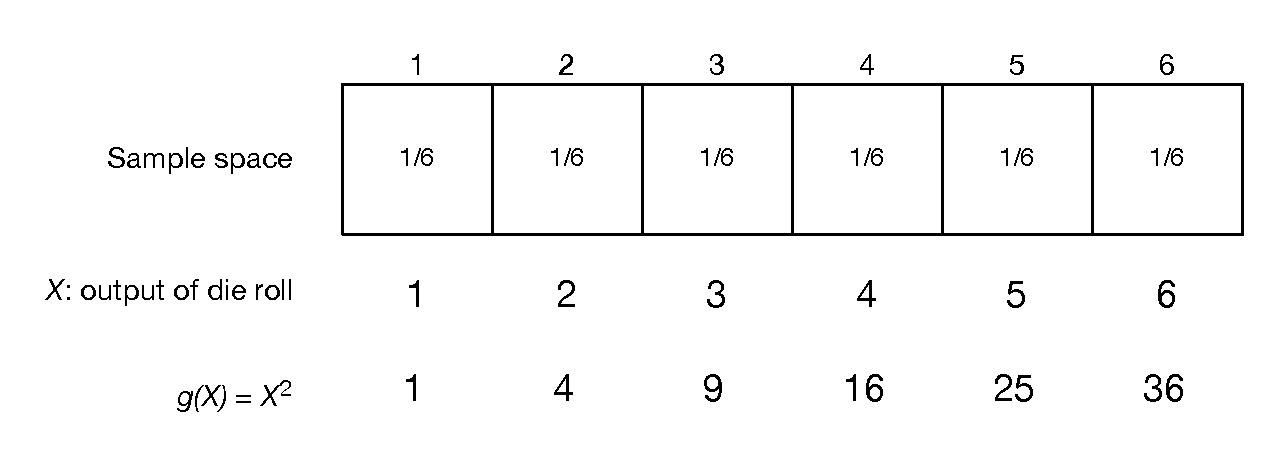
\includegraphics[width=10cm]{1diesquared}
\end{figure}
There are multiple ways to write the pmf for $g(X)$ in a table. I think the most useful way is to take the pmf table for $X$ and add an extra column for $g(X)$. We will see why this makes sense shortly.
\begin{figure}[H]
\centering
\begin{tabular}{l@{\hskip 2cm}l@{\hskip 2cm}l}
\toprule
$x$ & $g(x)$ & $p(x)$\\
\midrule
1 & 1 & 1/6\\
2 & 4 & 1/6\\
3 & 9 & 1/6\\
4 & 16 & 1/6\\
5 & 25 & 1/6\\
6 & 36 & 1/6\\
\bottomrule
\end{tabular}
\end{figure}

\end{example}

The expected value of a function of discrete random variable is computed in a similar fashion to the expected value of a random variable.

\begin{framed}
  \emph{Expected value of a function of a discrete random variable}\\
  \rule{\dimexpr\linewidth-2\fboxsep-2\fboxrule}{.1pt} \\
Let $Y$ be a discrete random variable with probability function $p(y)$, and let $g$ be a real-valued function. Then the expected value of the random variable $g(Y)$ is given by:
\[
\E[g(Y)] = \sum_{\text{all }y}g(y)\:p(y)
\]
where the sum is taken over all possible values $y$ can take. Note that the \emph{only} difference from the expected value of $Y$ is that we have $g(y)$ in place of $y$ in the sum. The probabilties $p(y)$ are \emph{unchanged}. This is again a weighted average, but this time we are taking a weighted average of the possible values of $g(Y)$.
\end{framed}

\begin{example}Let $X$ be the output of a standard six-sided die, and let $g(x) = x^2$. Find $E[g(X)]$.\\

We can use the formula for the expected value of a function of a random variable, together with the pmf table above to get:
\begin{align*}
\E[g(X)] &= \sum_{\text{all }x}g(x)\:p(x) \\
&= 1 \cdot \frac{1}{6} + 4 \cdot \frac{1}{6} + 9\cdot \frac{1}{6} + 16\cdot \frac{1}{6}+25\cdot \frac{1}{6}+36\cdot \frac{1}{6}\\
&= \frac{1}{6}(1 + 4 + 9 + 16 + 25 + 36)\\
&= \frac{91}{6} \approx 15.17
\end{align*}
\end{example}

Before we go on, we mention one more property of expected value: the expected value of a constant.

\begin{framed}
  \emph{Expected value of a constant}\\
  \rule{\dimexpr\linewidth-2\fboxsep-2\fboxrule}{.1pt} \\
Let $c$ be a constant. Then $\E(c) = c$. In other words, the expected value of a constant is just the constant itself. \\

We can combine this with the linearity of expectation to get the following. If $Y$ is a random variable, and $a$ and $b$ are constants, then
\[
\E(aY + b) = a\E(Y) + b
\]
\end{framed}

So far we have seen one quantititive descriptor of the distribution of a random variable: the expected value. Let's compare the pmfs of two discrete random variables.

\begin{example}Let $X$ be the number of heads observed when a fair coin is flipped 6 times, and let $Y$ be the uniform distribution on the integers $\{0, 1, 2, 3, 4, 5, 6\}$. Since $Y$ is the uniform distribution on a finite set with 7 elements, $\P(Y = y) = 1/7$ for all $Y$. $X$ takes the same values as $Y$ since the number of heads observed in 6 coin flips is an integer between 0 and 6. What is $\P(X = x)$? Since there are two possibilities for each flip, there are $2^6$ possible flip-sequences. The number of flip-sequences which give us $x$ heads is given by the binomial coefficient $\binom{6}{x}$ (why is this true?). Thus we have:
\[
\P(X = x) = \frac{\binom{6}{x}}{2^6}
\]
\end{example}
Putting both pmfs in tables we get:

\begin{figure}[H]
\centering
\begin{tabular}{l@{\hskip 2cm}l}
\toprule
$x$ & $p(x)$\\
\midrule
0 & 1/64\\
1 & 6/64\\
2 & 15/64\\
3 & 20/64\\
4 & 15/64\\
5 & 6/64\\
6 & 1/64\\
\bottomrule
\end{tabular}
\end{figure}

\begin{figure}[H]
\centering
\begin{tabular}{l@{\hskip 2cm}l}
\toprule
$y$ & $p(y)$\\
\midrule
0 & 1/7\\
1 & 1/7\\
2 & 1/7\\
3 & 1/7\\
4 & 1/7\\
5 & 1/7\\
6 & 1/7\\
\bottomrule
\end{tabular}
\end{figure}

Now let's look at the pmfs as histograms:
\begin{figure}[H]
\centering
\includegraphics[width=7cm]{excelx.pdf}
\includegraphics[width=7cm]{excely.pdf}
\end{figure}

Both of these two random variables have an expected value (mean) of 3. (You can compute it yourself if you want, or reason that both distributions are symmetric, and the ``middle'' is 3.) Despite having the same mean, the two distributions are very different. $X$ is relatively centered about the mean, while $Y$ is all ``spread out''. We want a way to quantify this amount of ``spread''. There are many ways to do this. For example, we could use the average distance from the mean. Statisticians have settled on a slightly different measure of ``spread'': the variance. In words, the variance of a random variable is the expected value of the squared-difference from the mean. Mathematically, we have the following definition:

\begin{framed}
  \emph{Variance of a discrete random variable}\\
  \rule{\dimexpr\linewidth-2\fboxsep-2\fboxrule}{.1pt} \\
Let $Y$ be a discrete random variable with probability function $p(y)$, and let $\mu = \E(Y)$ be its expected value (mean). Then we define the \emph{variance} of $Y$ by
\[
Var(Y) = \E[ (Y - \mu)^2 ]
\]
Using the formula for the expected value of a function of a random variable, this becomes
\[
Var(Y) = \sum_{\text{all }y}(y - \mu)^2 \:p(y)
\]
The variance is sometimes denoted by the symbol $\sigma^2$. The \emph{standard deviation} of a random variable is the square root of the variance, and is denoted $\sigma$.
\end{framed}

Let's compute the variance of the two random variables above. Since $Y$ is more ``spread out'' than $X$, we expect it to have a higher variance.

\begin{example}Let $X$ be the number of heads observed when a fair coin is flipped 6 times, and let $Y$ be the uniform distribution on the integers $\{0, 1, 2, 3, 4, 5, 6\}$. Compute the variances of both random variables.\\

The mean of both random variables is 3, so we have:
\begin{align*}
Var(X) &= \sum_{\text{all }x}(x - 3)^2 \:p(x) \\
&= (0-3)^2 \frac{1}{64} + (1-3)^2 \frac{6}{64} + (2-3)^2 \frac{15}{64} + (4-3)^2 \frac{20}{64} + (4-3)^2 \frac{15}{64} + (5-3)^2 \frac{6}{64} + (6-3)^2 \frac{1}{64} \\
&= \frac{(9)(1)}{64} + \frac{(4)(6)}{64} + \frac{(1)(15)}{64} + \frac{(0)(20)}{64} + \frac{(1)(15)}{64} + \frac{(4)(6)}{64} + \frac{(9)(1)}{64} \\ 
&= \frac{96}{64} \\
&= \frac{3}{2}
\end{align*}

\begin{align*}
Var(Y) &= \sum_{\text{all }y}(y - 3)^2 \:p(y) \\
&= (0-3)^2 \frac{1}{7} + (1-3)^2 \frac{1}{7} + (2-3)^2 \frac{1}{7} + (4-3)^2 \frac{1}{7} + (4-3)^2 \frac{1}{7} + (5-3)^2 \frac{1}{7} + (6-3)^2 \frac{1}{7} \\
&= \frac{1}{7}(9 + 4 + 1 + 0 + 1 + 4 + 9) \\
&= \frac{28}{7} \\
&= 4
\end{align*}
As predicted from the histograms, $Y$ has a much higher variance.
\end{example}

The variance is often not computed by using the definition above, but by using a formula affectionately known as the \emph{Magic Variance Formula}.

\begin{framed}
  \emph{Magic Variance Formula}\\
  \rule{\dimexpr\linewidth-2\fboxsep-2\fboxrule}{.1pt} \\
Let $Y$ be a random variable and let $\mu = \E(Y)$ be its expected value (mean). Then the variance of $Y$ is given by
\[
Var(Y) = \E[ Y^2 ] - \mu^2
\]
\end{framed}
To verify this formula, we expand out the binomial in the definition of variance, and use linearity of expectation.
\begin{align*}
Var(Y) &= \E[ (Y - \mu)^2] \\
&= \E( Y^2 - 2 \mu Y + \mu^2 ) \\
&= \E(Y^2) - 2 \mu \E(Y) + \E(\mu^2) \\
&= \E(Y^2) - 2 mu^2 + \mu^2 \\
&= \E(Y^2) - \mu^2
\end{align*}
where we used the fact that $\E(Y) = \mu$, and the expected value of a constant is just the constant.


\subsection{Bernouilli Trials}


\end{example}


\end{document}